\documentclass{article} 

\usepackage{amsmath,amsthm,amssymb,graphicx}

\graphicspath{ {C:/Users/David/SkyDrive/School/COMP 360/Assignments/} }

\newtheorem{problem}{Problem} 

\theoremstyle{definition} 

\newtheorem*{solution}{Solution} 

\begin{document} \title{Assignment 4} 

\author{Yang David Zhou, ID 260517397} 

\date{\today}

\maketitle

\begin{problem} 

Backtracking: Vertex Colouring.

\end{problem}

\begin{solution}

The colouring I found was A=1, B=2, C=1, D=3, E=2, F=3, G=2

\end{solution}

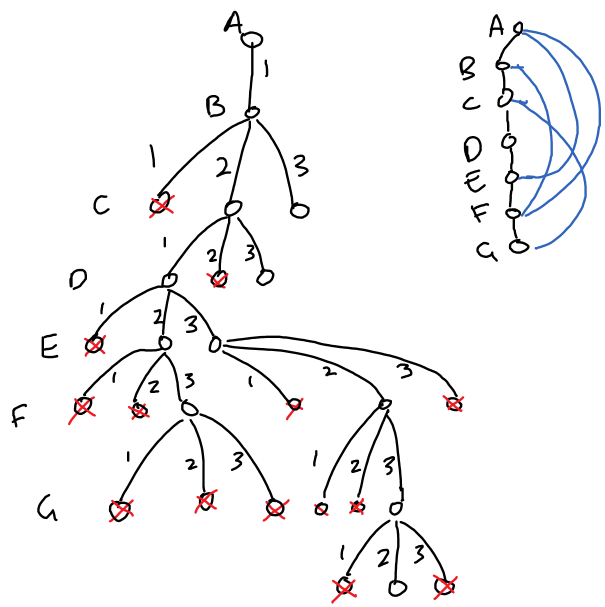
\includegraphics[scale=1]{a3q1} \\

\begin{problem} 

Local Search: Matching

\end{problem}

\begin{solution}

(a)  If the algorithm chooses the one of the two horizontal red edges on the left, then it will not find the maximum matching which is the three diagonal edges on the right.

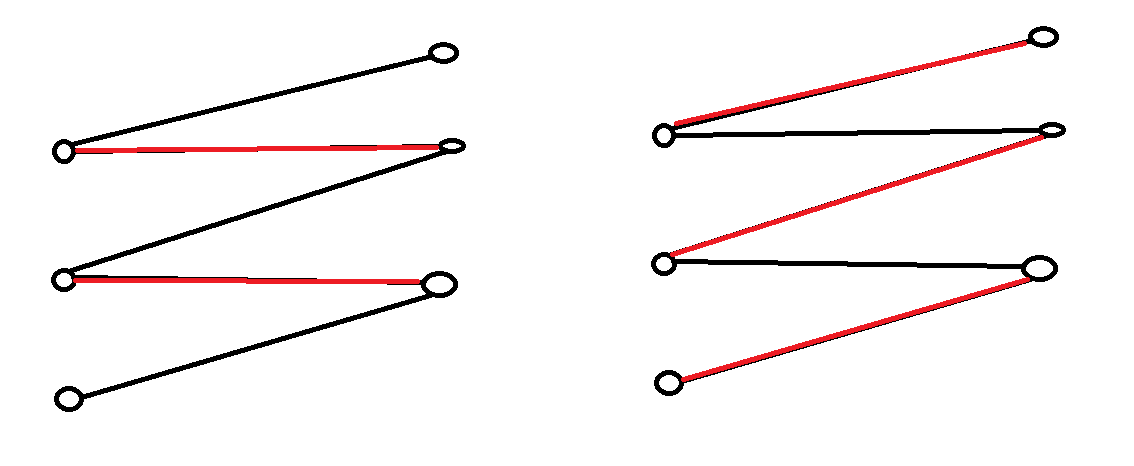
\includegraphics[scale=0.3]{a3q2a} \\

(b) Let \(A=M\cup M'\). There are now some \(k\) number of connected components \(C_1,...C_k\subseteq A\). Every \(e'_i\in M'\) can share end points with at most 2 edges \(e_i, e_j \in M\) and form a \(C_i\) which gives the constraint \(|M'|\leq 2|M|\), but it is given that \(|M'|>2|M|\), so there must exist some \(C_j\) such that \(C_j\cap M=\emptyset\) where \(C_j\) is an \(e'\in M'\) that can be added to \(M\) that maintains the bipartite property of \(M\). \\

(c) If \(M\) were the maximum matching of \(G={V,E}\) and \(M'\) the gradient ascent algorithm matching, then we know that there is no \(e\in E\) and so, no \(e\in M\) that can be added to \(M'\) by the algorithm definition. Thus, by the constraint found in (b), we have \(|M'|\geq \frac{1}{2}|M|\).

\end{solution}

\begin{problem} 

Local Search: Machine Scheduling.

\end{problem}

\begin{solution}

(a) At the conclusion of the algorithm there might be a machine with a smaller total time \(M_s\) and a machine with larger total time \(M_l\). There must be at least 2 jobs on \(M_l\). This is because it is given that the largest job \(t_j\) does not take more than half the total time of all jobs, i.e. \(t_j\leq  \frac{1}{2} (T_l+T_s) \).  The smallest job \(t_i\) on \(M_l\) was not moved to the other machine \(M_s\) so \(t_i\geq T_l-T_s\). If this is the case, then,

\(T_l-T_s\leq t_i \leq \frac{1}{2} (T_l+T_s) \)

\(T_l\leq t_i+T_s \leq \frac{1}{2} (T_l)+T_s \)

\(2\cdot T_l\leq 2(t_i+T_s) \leq T_l+2\cdot T_s \)

And if we ignore the middle inequality and subtract \(T_l\) from both sides,

\(T_l\leq 2\cdot T_s \)

Which is the given upper bound for the machine with the larger total time. \\

(b) For some job \(t_j\), it will only move if \(t_j<|T_1-T_2|\). Since \(|T_1-T_2|\) is always decreasing, after some number of moves, \(t_j\) will no longer move. Once the new rule for the choice of job is introduced, then \(t_j\) will  only be moved when it is the largest job. If \(t_j\) was the largest job then moving \(t_j\) will reduce \(|T_1-T_2|\leq t_j\). Thus \(t_j\) is only moved once. Since all jobs are only moved once, the maximum number of move operations is \(n\), the number of jobs. \\

(c) If \(M_1\) started with two jobs that are \(t=3\) each and \(M_2\) had four jobs with \(t=1\) each, then the algorithm will stop because no single job moved will not decrease \(|T_1-T_2|\). This result is not the globally optimal solution which is giving each of \(M_1\) and \(M_2\) one of the \(t=3\) jobs and two of the \(t=1\) jobs.

\end{solution}

\end{document}